
\documentclass[11pt]{report}


\usepackage[pdftex]{graphicx}
\usepackage{url} 
\usepackage[dvips, bookmarks, colorlinks=false, pdfborder={0 0 0}, pdftitle={<pdf title here>}, pdfauthor={<author's name here>}, pdfsubject={<subject here>}, pdfkeywords={<keywords here>}]{hyperref} 
\usepackage[final]{pdfpages}
\usepackage{multirow}
\usepackage[table]{xcolor} 

\title{XSM \\ eXperimental String Machine \\
Version 1.0}
\author{Dr. K. Muralikrishnan  \\ \texttt{kmurali@nitc.ac.in} \\ {NIT Calicut} }


\begin{document}

\maketitle
\pagebreak

%......................Table of Contents............................%
\thispagestyle{plain}

\tableofcontents
\pagebreak


\chapter{Introduction}

\section{Brief Machine Description}
The machine simulator is known as Experimental String Machine (XSM). It is an interrupt driven uniprocessor machine. The machine handles data as strings. A string is a sequence of characters terminated by '\textbackslash 0'. The length of a string is at most 16 characters including '\textbackslash 0'. Each of these strings is stored in a \textbf{word}  (Refer Section \ref{sec:mem}). The machine interprets a single character also as a string.

\section{Components of the Machine}

\begin{figure}[hbtp]
\begin{center}
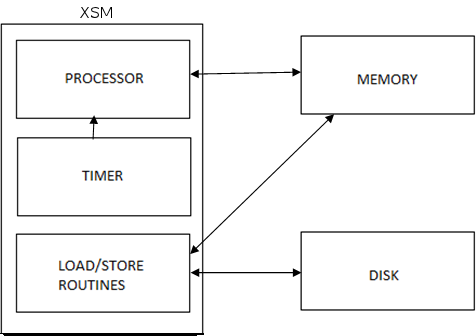
\includegraphics[scale=0.5]{block.png}
\end{center}
\caption{Components of the Machine}
\end{figure}

\begin{itemize}
\item \textbf{Disk} : It is a non-volatile storage that stores user programs (executables) and data files. The Operating System code is also stored in the disk.

\item \textbf{Memory} : It is a volatile storage that stores the programs to be run on the machine as well as the operating system that manages the various programs.
\item \textbf{Processor} : It is the main computational unit that is used to execute the instructions.
\item \textbf{Timer} : It is a device that interrupts the processor after a pre-defined specific time interval.
\item \textbf{Load/Store} : It is a macro that performs the functionalities of DMA (Direct Memory Access) controller. (Refer Section \ref{sec:inst})
\end{itemize}


\section{Supported Datatypes}

XSM supports 2 different datatypes and their operations, namely \textbf{Strings} and \textbf{Integers}. However in the lowest level both integers and strings are internally stored as strings.

\subsection{Strings} Strings are sequence of characters which may include alphabets, numerals and special characters. Every string is terminated with a \textit{null character} ('\textbackslash 0'). Operations that can be performed on strings include lexicographic comparisons.

\subsection{Integers} Apart from strings, XSM supports integers and its operations. The operations that can be performed on integers include arithmetic operations and comparison operations. A jump can also performed by checking if a register has 0 in it.



\chapter{Registers}

\section{Introduction}

The XSM architecture maintains 26 registers (each one \textbf{word}).

\section{Register Set}
There are 16 General Purpose Registers (GPR), \texttt{R0 - R15}, of which \texttt{R0 - R7} are Program Registers and \texttt{R8 - R15} are Kernel Registers. There are 4 temporary registers \texttt{T0 - T3} which are reserved for code translation. The registers \texttt{T0 - T3} are not intended to be used by the system programmer. In addition to these 20 registers there are 6 Special Purpose Registers(SPR) namely \texttt{BP} (Base Pointer), \texttt{SP} (Stack Pointer),  \texttt{IP} (Instruction Pointer), \texttt{PTBR} (Page Table Base Register) and \texttt{PTLR} (Page Table Length Register) and the \texttt{EFR} (Exception Flag Register)



\begin{center}
\begin{tabular}{|c|c|}
\hline Name & Register \\ 
\hline Program Register & R0-R7 \\ 
\hline Kernel Register & R8-R15 \\ 
\hline Temporary Registers & T0-T3 \\ 
\hline Base Pointer & BP \\ 
\hline Instruction Pointer & IP \\ 
\hline Stack Pointer & SP \\ 
\hline Page Table Base Register & PTBR \\
\hline Page Table Length Register & PTLR \\
\hline Exception Flag Register & EFR \\
\hline
\end{tabular} 
\end{center}


\chapter{Memory}
\label{sec:mem}

\section{Introduction}

%\begin{figure}[hbtp]
%\begin{center}
%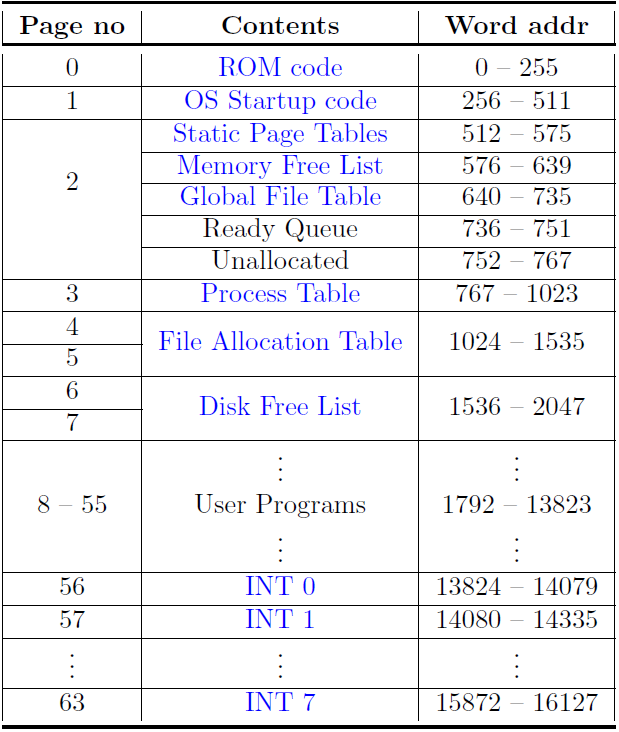
\includegraphics[scale=0.5]{memoryblockdiagram.png}
%\end{center}
%\caption{Main Memory Block Diagram}
%\end{figure}

\begin{itemize}
\item The basic unit of memory in XSM is a \textbf{word} (length = 16 bytes).
\item The machine memory can be thought of as a linear sequence of \textbf{words}.
\item A collection of 512 contiguous \textbf{words} is known as a \textbf{page}.
\item The total size of the memory is 64 \textbf{pages} or 32768 (512 $\times$ 64) \textbf{words}.
\item Each \textbf{word} in the memory is identified by the \textit{word address} in the range 0 to 32767. Similarly, each \textbf{page} in the memory is identified by the \textit{page number} in the range 0 to 63.
\item The \textit{page number} corresponding to a word is obtained by the formula,
\begin{center}
 \textit{ page number }= $\lfloor \frac{word\ address}{512} \rfloor$
\end{center}
\end{itemize}



\section{Address Translation}

There are two kinds of memory addresses,

\begin{itemize}
\item Logical address : When a process runs, CPU generates address for the data accessed by this process. This address is called the Logical address.

\item Physical address : It is the actual location of the data in the main memory.
\end{itemize}

Address translation is the process of obtaining the physical address from the logical address. It is done by the machine in the following way. 
\begin{enumerate}
\item The logical address generated by the CPU is divided by the page size (512) to get the \textbf{logical page number}. The remainder is the \textbf{offset} of the data within that page.


\item A \textbf{page table} is used for address translation. It resides in the memory, the location of which is pointed to by \textbf{PTBR} (Page Table Base Register
). The number of entries in the page table is stored in \textbf{PTLR} (Page Table Length Register). Each entry of the page table is two words long.
\begin{itemize}
 \item[--] First word contains physical page number corresponding to a logical page number.
 \item[--] The second word can be used as flags. The first two positions in this word is used as \textit{valid/invalid bit} (if the entry is a valid physical memory location or not) and \textit{reference bit} (its set to 1 every time a page is accessed) respectively.
 	
\end{itemize}
The logical page number is used to index the page table to get the corresponding physical page number.

\item The \textbf{offset} is then used to refer to the word in the physical page containing the data.
\end{enumerate} 
\vspace{0.3in}

The example below shows the address translation corresponding to the logical address  13532.
\begin{figure}[ht]
	\centering
	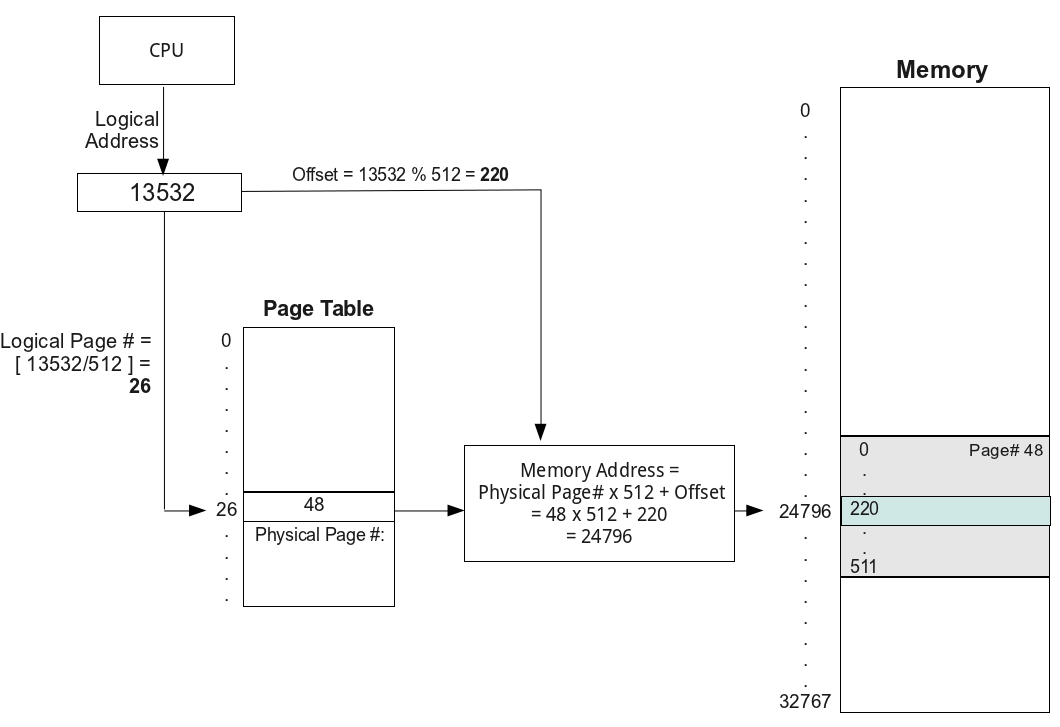
\includegraphics[scale=0.35]{address_translation.png}
	\caption{ \small The logical address generated by the CPU is 13532, so the page number is $\lfloor 13532/512 \rfloor$ = 26 and offset is 13532 mod 512 = 220. Let the 26$^{th}$ entry in the page table be 48. Thus the resultant physical address is 48 $\times$ 512 + 220 = 24796.}
	\label{fig:paging}
\end{figure}


\section{ROM Code}
\label{lbl:romcode}
It is a hard coded assembly level code present in page 0 of the memory. It is known as the ROM (Read Only Memory) code because in an actual machine it is burnt in the hardware. When the machine boots up, this code is executed. This code has the basic functionality of loading block 0 of the disk (which generally contains the OS startup code) into page 1 of the memory and to set the \texttt{IP} register value to 512.



\chapter{Disk Storage}


\textbf{Block} : It is the basic unit of storage in the disk.\\

The disk can be thought of as consisting of a linear sequence of 512  \textbf{blocks}. The size of each \textbf{block} is equal to that of a page in the memory (512 words). The total disk capacity is 512 $\times$ 512 = 262144 \textbf{words}.\\

Any particular \textbf{block} in the disk is addressed by the corresponding number in the sequence 0 to 511 known as the \textit{block number}.

\begin{figure}[htp!] \small
	\centering
	\begin{tabular}{|c|c|c|c|} 
	\hline
       0 - 511 & 512 - 1023 & ... &   261632 - 262143     \\
       \hline      
      & & & \\ 
      Block 0 & Block 1  & .... & Block 512 \\ 
      & & & \\       
       \hline
       
	\end{tabular}
	\caption{Disk Structure}
	\label{fig:mem_struct}
\end{figure}




 \chapter{Instructions}
\label{sec:inst}
\section{Introduction}

Every instruction in XSM is 2 words long. The instructions provided by the XSM architecture can be classified into privileged and unprivileged instructions.

\section{Classification}

\subsubsection{Unprivileged Instructions}

\begin{enumerate}
\item \texttt{MOV}
\begin{itemize}

\item Register Addressing:\\
\textit{Syntax :} \texttt{MOV Ri, Rj}\\
Copies the contents of the register \texttt{Rj} to \texttt{Ri}.

\item Immediate Addressing:\\
\textit{Syntax :} \texttt{MOV Ri, INTEGER/STRING}
Copies the \texttt{INTEGER/STRING} to the register \texttt{Ri}.


\item Register Indirect Addressing:\\
\textit{Syntax }: \texttt{MOV Ri, [Rj]}\\
Copy contents of memory location pointed by \texttt{Rj} to register \texttt{Ri}.\\
\textit{Syntax :}\texttt{ MOV [Ri], Rj} \\
Copy contents of \texttt{Rj} to the location whose address is in \texttt{Ri}.


\item Direct Addressing:\\
\textit{Syntax :}\texttt{ MOV [LOC], Rj}\\
Copy contents of \texttt{Rj}  to the memory address \texttt{LOC}.\\
\textit{Syntax :} \texttt{MOV Rj, [LOC]}\\
Copy contents of the memory location \texttt{LOC} to the register \texttt{Rj}.

\item Direct Indexed Addressing: \\
\textit{Syntax :}\texttt{ MOV [LOC] Rj, Ri}\\
Copy contents of \texttt{Ri} to the memory address \texttt{LOC} + (value in \texttt{Rj}) \\
\textit{Syntax :}\texttt{ MOV [LOC] Index, Rj}\\
Copy contents of \texttt{Ri} to the memory address \texttt{LOC} + \texttt{Index}. \texttt{Index} must be an integer value. \\
\textit{Syntax :}\texttt{ MOV Ri, [LOC] Rj}\\
Copy contents in the memory address \texttt{LOC} + (value in \texttt{Rj}) to the register \texttt{Ri}\\
\textit{Syntax :}\texttt{ MOV Ri, [LOC] Index}\\
Copy contents of the memory address \texttt{LOC} + \texttt{Index} to the register \texttt{Ri}. \texttt{Index} must be an integer value. \\
\end{itemize}


\item\textbf{ Arithmetic Instructions}
\\
Arithmetic Instructions perform arithmetic operations on registers containing integers. If the register contains a non-integer value, an exception is raised (Refer Section \ref{exception})
\begin{itemize}
\item \texttt{ADD}, \texttt{SUB}, \texttt{MUL}, \texttt{DIV} and \texttt{MOD}.\\
\textit{General Syntax :} \texttt{OP Ri, Rj}\\
The result of \texttt{Ri} op \texttt{Rj} is stored in \texttt{Ri}. 

\item \texttt{INR\\}
\textit{Syntax :}\texttt{ INR Ri}\\
Increments the value of register \texttt{Ri} by 1.  

\item  \texttt{DCR}\\
\textit{Syntax :} \texttt{DCR Ri}\\
Decrements the value of register \texttt{Ri} by 1. 

\end{itemize}


\item \textbf{Logical Instructions} \\
Logical instructions are used for comparing values in registers. Strings can also be compared according to the lexicographic ordering of ASCII.
\begin{itemize}

\item \texttt{LT}\\
Syntax :\texttt{ LT Ri, Rj}\\
Stores 1 in \texttt{Ri} if the value stored in \texttt{Ri} is less than that in \texttt{Rj}. \texttt{Ri} is set to 0 otherwise. 

\item \texttt{GT}\\
Syntax : \texttt{GT Ri, Rj}\\
Stores 1 in \texttt{Ri} if the value stored in \texttt{Ri} is greater than that in \texttt{Rj}. \texttt{Ri} set to 0 otherwise. 

\item \texttt{EQ}\\
Syntax : \texttt{EQ Ri, Rj}\\
Stores 1 in \texttt{Ri} if the value stored in \texttt{Ri} is equal to that in \texttt{Rj}. Set to 0 otherwise. 

\item \texttt{NE}\\
Syntax : \texttt{NE Ri, Rj}\\
Stores 1 in \texttt{Ri} if the value stored in \texttt{Ri} is not equal to that in \texttt{Rj}. Set to 0 otherwise. 

\item \texttt{GE} \\
Syntax : \texttt{GE Ri, Rj} \\
Stores 1 in \texttt{Ri} if the value stored in \texttt{Ri} is greater than or equal to that in \texttt{Rj}. Set to 0 otherwise. 

\item \texttt{LE}\\
Syntax : \texttt{LE Ri, Rj}\\
Stores 1 in \texttt{Ri} if the value stored in \texttt{Ri} is less than or equal to that in \texttt{Rj}. Set to 0 otherwise. 
\end{itemize}


\item Branching Instructions
Branching is achieved by changing the value of the \texttt{IP} to the word address of the target instruction specified by \texttt{ $<$target\_address$>$ }. 
 
\begin{itemize}
\item \texttt{JZ}\\
Syntax : \texttt{JZ Ri, $<$target\_address$>$}\\
Jumps to \texttt{$<$target\_address$>$} if the contents of \texttt{Ri} is zero.
\item \texttt{JNZ}\\
Syntax : \texttt{JNZ Ri, $<$target\_address$>$}\\
Jumps to \texttt{$<$target\_address$>$} if the contents of \texttt{Ri} is not zero.
\item \texttt{JMP}\\
Syntax : \texttt{JMP $<$target\_address$>$}\\
Unconditional jump to \texttt{$<$target\_address$>$}\\

\end{itemize}

\item Stack Instructions
\begin{itemize}
\item \texttt{PUSH}\\
Syntax : \texttt{PUSH Ri}\\
Increment \texttt{SP} by 1 and copy contents of \texttt{Ri} to the location pointed to by \texttt{SP}.
\item \texttt{POP}\\
Syntax : \texttt{POP Ri}\\
Copy contents of the location pointed to by \texttt{SP} into \texttt{Ri} and decrement \texttt{SP} by 1.\\
For both these instructions \texttt{Ri} may be any register except \texttt{IP}.
\end{itemize}

\item Subroutine Instructions\\
The \texttt{CALL} instruction copies the address of the next instruction to be fetched on to location \texttt{SP} + 1. It also increments \texttt{SP} by one and transfers control to the instruction specified by the \texttt{$<$target\_address$>$}. The address of the instruction to be fetched is in \texttt{IP + 2} (each instruction is 2 memory words). The \texttt{RET} instruction restores the \texttt{IP} value stored at location pointed by \texttt{SP}, decrements \texttt{SP} by one and continues execution fetching the next instruction pointed to by \texttt{IP}. The subroutine instructions provide a neat mechanism for procedure evocations.
\begin{itemize}
\item \texttt{CALL}\\
Syntax : \texttt{CALL $<$target\_address$>$}\\
Increments \texttt{SP} by 1, transfers \texttt{IP}+2 to location pointed to by \texttt{SP} and jumps to instruction specified by $<$target\_address$>$
\item \texttt{RET}\\
Syntax : \texttt{RET}\\
Sets \texttt{IP} to the value pointed to by \texttt{SP} and decrements \texttt{SP}.
\end{itemize}

\item Input/Output Instructions
\begin{itemize}
\item \texttt{IN}\\
Syntax : \texttt{IN Ri}\\
Transfers the contents of the standard input to \texttt{Ri}.
\item \texttt{OUT}\\
Syntax : \texttt{OUT Ri}\\
Transfers the contents of \texttt{Ri} to the standard output.\\
\end{itemize}


\item Debug Instruction\\
Syntax : \texttt{BRKP}\\
Displays contents of all registers and memory locations at the time when the instruction is invoked. This instruction can be used for debugging system code.


\item \texttt{END}\\
Syntax : \texttt{END}\\
This instruction is marks the end of a program.

\item \texttt{INT}\\
Syntax : \texttt{INT n}\\
Generates an interrupt to the kernel with \texttt{n} (1 to 6) as a parameter. It also disables the interrupts. (Read Section \ref{sec:int})



\end{enumerate}


\subsubsection{Privileged Instructions}
There are four privileged instructions. They can only be executed in kernel mode (Refer to \ref{sec:priv_modes}).  These instructions are:
\begin{enumerate}

\item \texttt{IRET}\\
Syntax : \texttt{IRET}\\
\texttt{IRET} switches the mode from kernel to user mode. It then sets \texttt{IP} to the value pointed by \texttt{SP} and decrements \texttt{SP} by one. With the execution of the \texttt{IRET} instruction, interrupts are enabled. (Read Section \ref{sec:int})

\item \texttt{LOAD}\\
Syntax : \texttt{LOAD \textit{pagenum} \textit{blocknum}}\\
This instruction loads the block specified by the \texttt{\textit{blocknum}}, from the disk, to the page specified by the \texttt{\textit{pagenum}} in the memory. \texttt{\textit{blocknum}} and \texttt{\textit{pagenum}} should be numbers or registers containing numbers. An excpetion is raised (Refer Section \ref{exception}) for invalid arguments or illegal memory access.

\item \texttt{STORE}\\
Syntax : \texttt{STORE \textit{blocknum} \textit{pagenum} }\\ 
This instruction stores the page specified by the \texttt{\textit{pagenum}}, from the memory, to the block specified by the \texttt{\textit{blocknum}}in the disk. \texttt{\textit{blocknum}} and \texttt{\textit{pagenum}} should be numbers or registers containing numbers. An excpetion is raised (Refer Section \ref{exception}) for invalid arguments or illegal memory access.\\

The below example will store the 31st page in memory to the 64th block in the disk. It will then load it to the 15th page in memory.
\begin{verbatim}
MOV R1, 64
STORE R1, 31
LOAD 15, R1	
\end{verbatim}	

\item \texttt{HALT}\\
Syntax : \texttt{HALT}\\
This instruction causes the machine to halt immediately. 
\end{enumerate}

\section{Privilege Modes}
\label{sec:priv_modes}
The XSM architecture is interrupt driven and uses a single processor. There are two privilege modes of execution, the user mode and the kernel mode. The machine is initially in kernel mode. It switches to user mode when it encounters an IRET instruction. It switches back to kernel mode after an interrupt or an exception occurs.


\begin{itemize}
\item User mode : Only unprivileged instructions can be executed in this mode. Only registers \texttt{R0} to \texttt{R7}, \texttt{SP} and \texttt{BP} are allowed to be used in any instruction in this mode. Address translation occurs for all addresses in user mode.

\item Kernel mode : Both privileged and unprivileged instructions can be executed in this mode. The value of \texttt{IP} and \texttt{EFR} cannot be explicitly changed by any instruction. Also these registers cannot be used in addressing memory locations. All other registers can be used in Kernel Mode. Address translation does not occur in kernel mode. 


\end{itemize}

\chapter{Interrupts}
\label{sec:int}

Interrupts are mechanisms by which the machine interrupts the execution of the processor and passes control to the kernel to execute interrupt (or exception) handler code. Interrupts might indicate errors, such as a memory access violation (page fault), a timer interrupt or a software interrupt invocation from a running program. \\

The process saves its current state before starting execution of the handler, and then resumes the state once the handler finishes its execution. Interrupts are disabled when the interrupt handler code is executing. 


\section{Exceptions}
\label{excpetion}
Exceptions are anomalous situations which changes the normal flow of execution. There is a flag associated with each exception and the details corresponding to the exception that occured is stored in \texttt{EFR}. If an exception occurs in User Mode, the machine transfers control of execution, i.e. changes the value of IP to \textit{page number} 7 (address = 3584) where the Exception Handler Routine resides. However in Kernel Mode, the machine halts when it encounters an exception. \\

The structure of \texttt{EFR} is given below
		\begin{figure}[htp!]
		\centering
		\begin{tabular}{|c|c|c|c|}
		\hline
		\texttt{Value of IP} & \texttt{BadVAddr} & \texttt{Cause} &  \textbackslash 0 \\
		\hline
		\end{tabular}
		\end{figure}

\begin{itemize}
\item \textbf{Value of IP}: Stores the value of IP at the point where the exception occured. The maximum length of IP is 5 digits.
\item \textbf{BadVAddr} (Bad Virtual Address). This field is relevant when a Page Fault Exception occurs. The logical page number which caused a page fault exception is stored here. The length of this field is 2 characters.
\item \textbf{Cause}: This field indicates a number which corresponds to the cause of the exception. 
eg : a page fault exception has value 0 stored in Cause field. The length of this field is 1 character.
\end{itemize}

Exceptions can be caused when the following events occur.

\begin{enumerate}
\item \textbf{Page Fault} : occurs when the page table entry corresponding to the logical address is invalid. The value stored in \textit{cause} field of \textbf{EFR} for this exception is \textbf{0}.

\item \textbf{Illegal instruction} : occurs when an attempt is made to execute an instruction not belonging to the instruction set and also when the operands to the instruction is not legal. Eg: \texttt{MOV 4 R0}, \texttt{MOV IP 4} when executed in user mode. These instructions are considered illegal. The value stored in the \textit{cause} field of \textbf{EFR} for this exception is \textbf{1}.

\item \textbf{Illegal memory access} : occurs when any address generated by the process lies outside its logical address space. The logical page number generated should be between 0 and the value of \texttt{PTLR}.  The value stored in the \textit{cause} field of \textbf{EFR} for this exception is \textbf{2}.

\item \textbf{Arithmetic exception} : occurs when divisor is 0. The value stored in the \textit{cause} field of \textbf{EFR} for this exception is \textbf{3}.

\item \textbf{Illegal operands} : occurs when operands contain invalid data corresponding to the instruction. The value stored in the \textit{cause} field of \textbf{EFR} for this exception is \textbf{4}.


\end{enumerate}

\section{Timer Interrupt }
Timer Interrupt is generated by the machine, usually at set timer intervals. This interrupt cannot be invoked from the user/kernel mode.\\

It transfers control of execution, i.e. changes the value of IP to \textit{page number} 8 (address = 4096). This is the timer interrupt which interrupts the processor. Generally it is supposed to contain the code for the scheduler of the operating system, which schedules the CPU time among the various active processes.

\section{Software Interrupts }
Software Interrupts interrupts are unprivileged and can be called from user mode. 7 Interrupt instructions are provided by the machine which causes the execution of ISR (Interrupt Service Routines) in 7 different pages in the memory. 

\subsubsection{The \texttt{INT} instruction}
The instruction used to generate a software interrupt is \texttt{INT}.\\
Syntax : \texttt{INT n}\\
The \texttt{INT} instruction passes control to the Interrupt Service Routine (ISR) for this interrupt located at the physical address computed using the value n. The physical address of the ISR corresponding to interrupt number n is given by: 
\begin{verbatim}
Physical Address = (8 + n) x Page Size
\end{verbatim}
Note that the interrupts are disabled once this instruction is executed as interrupts cannot be executed in kernel mode.\\

The 7 \texttt{INT} instructions are :
\begin{itemize}

\item \texttt{INT 1}  \\It transfers control of execution to \textit{page number} 9 (address = 4608)
\item \texttt{INT 2}  \\It transfers control of execution to \textit{page number} 10 (address = 5120)  
\item \texttt{INT 3}  \\It transfers control of execution to \textit{page number} 11 (address = 5632)
\item \texttt{INT 4}  \\It transfers control of execution to \textit{page number}  12 (address = 6144) 
\item \texttt{INT 5}  \\It transfers control of execution to \textit{page number} 13 (address = 6656)
\item \texttt{INT 6}  \\It transfers control of execution to \textit{page number} 14 (address = 7168)
\item \texttt{INT 7}  \\It transfers control of execution to \textit{page number} 15 (address = 7680).\
 
\end{itemize}

Brief memory outline for XSM is given below.
\begin{center}
\begin{tabular}{|c|c|c|}
\hline \textbf{Page Number} & \textbf{Contents} & \textbf{Word Address}  \\ 
\hline 0 & ROM Code &  0 -- 511\\ 
1 & OS Startup Code & 512 -- 1023 \\ 
2 -- 6 & OS Structures  &  1024 -- 3583\\ 
 \rowcolor{gray!15}
\hline 7 & Exception Handler  &  3584 -- 4095\\ 
 \rowcolor{gray!15}
 8 & Timer Interrupt Routine  &  4096 -- 4607\\ 
 \rowcolor{gray!15}
 9 & Interrupt 1  &  4608 -- 5119\\ 
 \rowcolor{gray!15}
10 & Interrupt 2  &  5120 -- 5631\\ 
 \rowcolor{gray!15}
 11 & Interrupt 3  &  5632 -- 6143\\ 
 \rowcolor{gray!15}
 12 & Interrupt 4  &  6144 -- 6655\\ 
 \rowcolor{gray!15}
 13 & Interrupt 5  &  6656 -- 7167\\ 
 \rowcolor{gray!15}
 14 & Interrupt 6  &  7168 -- 7679\\
 \rowcolor{gray!15} 
 15 & Interrupt 7  &  7680 -- 8191\\ 
\hline 16 -- 63 & User Programs & 8192 -- 32767\\
\hline
\end{tabular} 
\end{center}


\end{document}
